\chapter{High Intensity Studies}
\label{sec:ch6}

\section{Space Charge Tune Shift}

For this chapter, the focus goes back to the Fermilab Recycler Ring. All the experiments and measurements done in Ch. \ref{sec:ch4} were done at low intensities, i.e., less than 1e10 particles per bunch (ppb). Nevertheless, current operations and future operations under PIP-II objectives are done at higher intensities, i.e., 5e10 ppb for current operations and 8e10 ppb for PIP-II. Therefore, it is relevant to explore resonance compensation at higher intensities. 

An important parameter for high-intensity operation is the space charge tune shift. As mentioned in Ch. \ref{sec:ch2}, the space charge tune shift is an incoherent quantity meaning every particle will feel a different magnitude of this effect. Nevertheless, as shown in Figs. \ref{fig:rrtdmid} and \ref{fig:rrtdhigh}, this incoherent quantity will be contained within a necktie distribution. This necktie profile will define the space charge tune spread. When particles are in the beam core, they will feel the largest space charge potential, leading to the largest detuning and defining the edge of the necktie distribution.

Equation \ref{eq:scave1} showed a general way to calculate the space charge tune shift for particles at different amplitudes $J_u$. Nevertheless, this calculation is an involved process where the envelope equation has to be solved around the ring at the same time as the Poisson equation, Eq. \ref{eq:poisson1}. Different approximations can be done, in order to do rapid estimates of the space charge tune shift. Furthermore, a more important quantity is the maximum tune shift of the beam core particles. This will ultimately define the space charge tune spread. While this quantity can be calculated using PySCRDT \cite{scrdt_report}, a cruder estimate can also be calculated. This involves using a smooth-lattice approximation and circular beam pipe approximation, as used in Ref. \cite{zhang}. 

With these simplifications, the space charge tune spread can be found as:
\begin{equation}
    \label{eq:tunesc}
    \Delta Q_{u,sc}=\frac{-3 N_b r_0 R S}{4 \sigma_z \beta_L \gamma_L ^2 \varepsilon_{n,u,95\%}},    
\end{equation}
where $N_b$ is the number of protons per bunch, $r_0=1.535\times 10^{-18}$ meters is the classical radius of the proton, $\sigma_z = 0.5726$ meters is the bunch length, $R = C/(2 \pi)$ is the radius of the Recycler Ring with a circumference of $C=3319.4$ meters, $S=1.596$ is a geometrical factor of the bunch, $\varepsilon_{n,u,95\%}$ is the 95\% normalized emittance in the $u$ plane, and $(\beta_L,\gamma_L)$ are the longitudinal relativistic factors. The following section explores a method in order to measure this tune spread.  

\section{Measurement of Tune Spread}

The $3Q_x=76$ line can be used to estimate the tune spread of beam in the Recycler Ring. As seen before, when a dynamic tune ramp is set and $3Q_x$ is crossed, 95\% of the beam is lost. By monitoring the tune ramp set into the tune trombone and assuming a linear tune ramp, one can correlate the tune instance when losses first appear with the tune spread. The tune distance between the losses first appearing and the $3Q_x$ line is a crude estimate for the tune spread. This is a crude estimate in the sense that particles in the beam core---particles with the largest tune shift---will start feeling the resonance and drift to higher amplitudes. The migration of particles from the beam core to the tails means that the tune shift will be smaller. There is a time delay (tune distance delay) between particles touching the resonance and particles being lost to the aperture. While this delay exists but given the large strength of the $3Q_x$ line, just hitting the resonance head on can still give a crude estimate for the value of the tune spread and its behavior.

Figure \ref{fig:dynamictunespread} shows slices of loss maps at different intensities used in order to measure this tune spread. The top slice corresponds to an intensity of 2 Booster Turns (BTs), i.e., approximately $0.6\times10^{10}$ particles per bunch for this particular experiment. The bottom slice corresponds to an intensity of 17 BTs, approximately $6.0\times10^{10}$ ppb, which is close to the maximum intensity that can be provided by Booster in single batch. The important thing to note here is that as the intensity increases the losses happen earlier in the tune ramp. This can be correlated to the space charge tune spread using the location of the $3Q_x$ line, which corresponds to where all the beam is lost. For example, for the bottom slice the losses start happening at $Q_x=25.36$, while all beam is lost at $Q_x=25.34$. This means the space charge tune spread can be approximated to 0.02. Ultimately, Fig. \ref{fig:dynamictunespread} shows beams with space charge tune spreads that range from 0.005 to 0.02.

\newpage
\begin{figure}[H]
    \centering
    \includegraphics[width=\textwidth,height=0.95\textheight,keepaspectratio]{chapter6/scts_measure.png}
    \caption{Dynamic loss strips at a fixed vertical set tune of $Q_y=24.45$ and on a range from $Q_x=25.39$ to $Q_x=25.32$ for different intensities.}
    \label{fig:dynamictunespread}
\end{figure}
\newpage

Another thing to note from Fig. \ref{fig:dynamictunespread} is how the space charge tune spread tends to stabilize to a value of around 0.02 for intensities higher than 12 BTs or $4.4\times 10^{10}$. This is due to the fact that the equilibrium emittance grows exponentially at higher intensities. Specifically, Ref. \cite{betiay} shows how the beam emittance grows with intensity in the Recycler Ring. It looks at the first turn emittance coming from the Booster Ring, which will dictate the initial tune shift of the Recycler Ring. This study combined with calculations of the space charge tune shift provided in Ref. \cite{zhang}, explain this behavior. The emittance grows exponentially as the beam intensity is increased, leading to a saturated tune shift value. Figure \ref{fig:tunespread} summarizes this behavior by plotting the measured tune spread from losses, the calculated tune spread from the first-turn abort emittance and, finally, the first-turn abort 95\% emittance on the right vertical axis.   

The maximum tune spread shown in Figs. \ref{fig:dynamictunespread} and \ref{fig:tunespread} is around 0.02, which only compares to 1/5 of the PIP-II projection. It is worth pointing out, that these experiments are done for a single batch with no slip stacking. Therefore, with slip stacking and smaller beam emittance coming from Booster, space charge tune shifts in the RR of around 0.1 will be possible in the PIP-II era. For now, Fig. \ref{fig:tunespread} shows how the tune spreads are not large enough to consider space-charge-dominated losses in the Recycler Ring relevant. All current losses are emittance-dominated, meaning the beam from Booster is hitting on the acceptance of the Recycler.  

\begin{figure}[H]
    \centering
    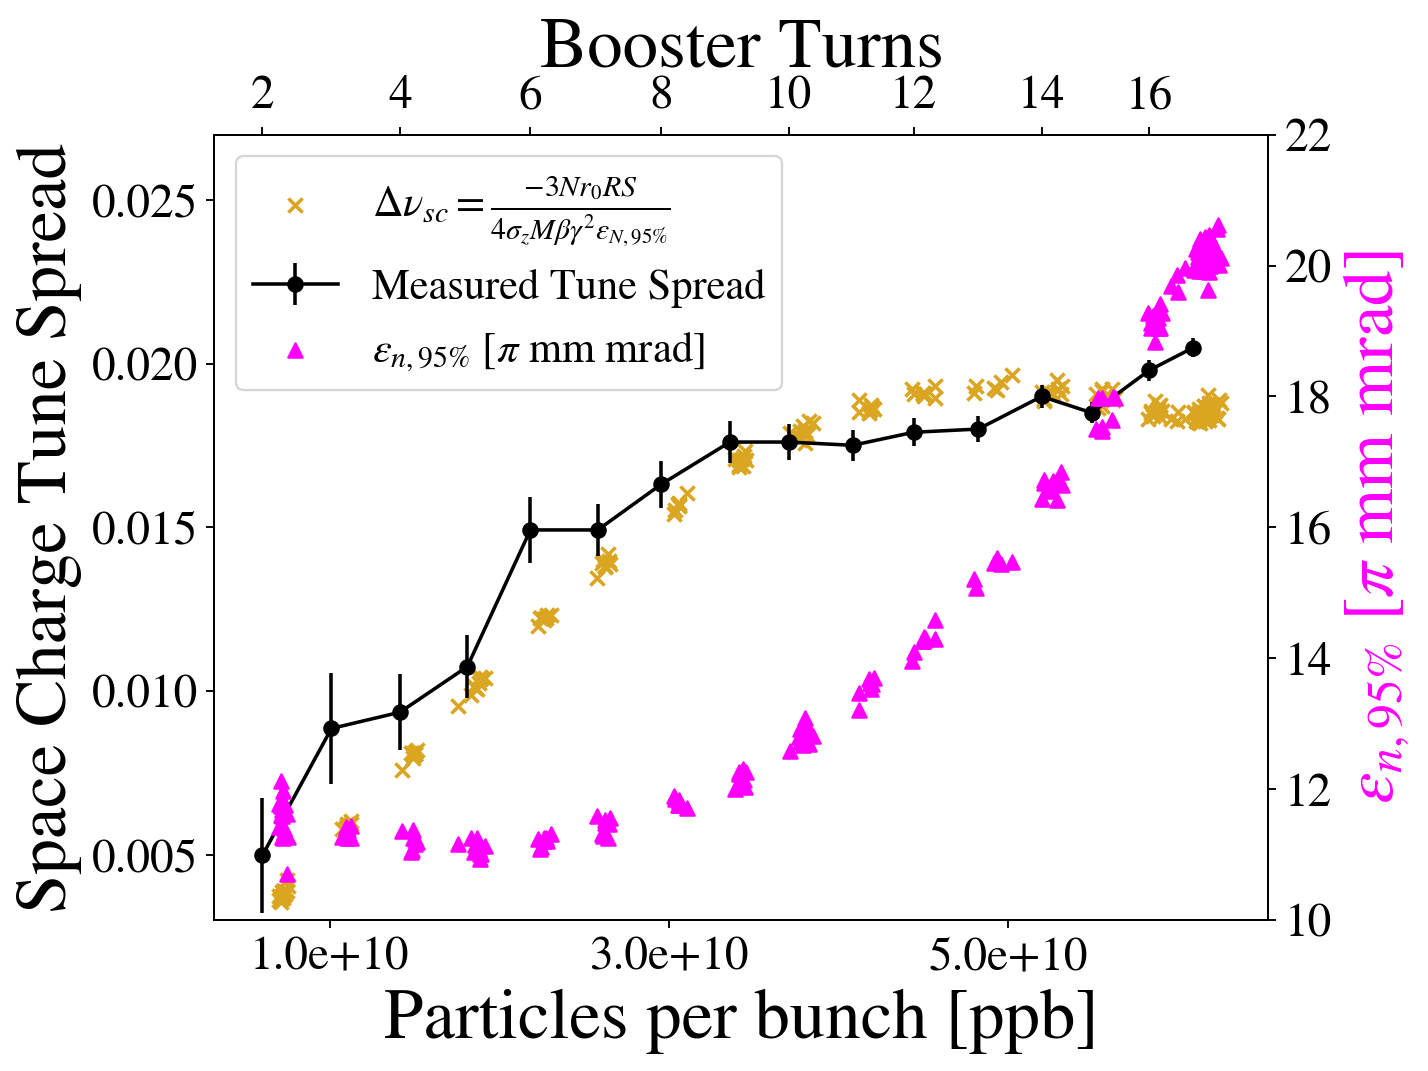
\includegraphics[width=\columnwidth]{chapter6/tune_spread.png}
    \caption{Tune spread measurements compared to tune spread calculations from horizontal emittances measured with multiwire data on first-turn abort beam.}
    \label{fig:tunespread}
\end{figure}

\section{\label{sec:qgaussian}Intensity-Dependent Effects and Non-Gaussian Beam Profiles}

As mentioned in Sec. \ref{sec:diagnostic}, the Ion Profile Monitor system is a useful tool to extract information about the transverse beam distribution. In particular, fitting a Gaussian distribution and extracting the scaling parameter or sigma $\sigma_u$ can help characterize the transverse beam size. Such as it was done in Figs. \ref{fig:static2_ipm} and \ref{fig:static2_ipm_comp}, the beam size growth can be correlated to the beam loss in the machine. Nevertheless, one can go a step further and look into deviations from Gaussian distributions. Reference \cite{nongaussian} looks into an application and explanation for this non-Gaussian profiles.

In particular, it is of interest to look at how the beam tails populate with incoming particles from the beam core. This happens when the space charge detuning is large enough for particles in the beam core to start touching resonances lines, and therefore migrate to larger amplitudes, i.e., the beam tails. In order to quantify this effect one can use q-Gaussian distributions \cite{nongaussian,qgaussian}. The definition for the probability density function $f_q(x)$ of this distribution for a given $q$ reads:
\begin{equation}
    \label{eq:qgaussian}
    f_q(x)=\frac{1}{\sigma C_q \sqrt{2}}e_q\left( -\frac{x^2}{2 \sigma^2}\right),
\end{equation}
where $\sigma$ is the scale parameter for the distribution and corresponds to the usual standard deviation of a Gaussian $\sigma$ when $q=1$. Additionally, $C_q$ is the normalization constant. The auxiliary function $e_q(x)$ is defined as:
\begin{equation}
    \label{eq:eqqGaussian}
    e_q(x)= \left\{
        \begin{array}{cl} 
            \exp{(x)}, & \text{if  } q = 1\\
            \left( 1+\left( 1-q \right)x\right)^{\frac{1}{1-q}}, & \text{if  } q \neq 1 \text{ and } \left( 1+\left( 1-q\right)x\right)>0\\
            0  & \text{if  } q \neq 1 \text{ and } \left( 1+\left( 1-q\right)x\right) \leq 0 
        \end{array} 
    \right.,
\end{equation}
where the usual Gaussian distribution is recovered when $q=1$. The distribution is said to have heavy tails when $q>1$, and light tails when $q<1$. The usual Gaussian distribution is recovered when $q=1$, and the usual Cauchy-Lorentzian distribution is recovered when $q=2$. Figure \ref{fig:qgaussians} shows a comparison of the probability density function for several values of $q$. It shows tails can become more populated for larger values of $q$ or under-populated for smaller values of $q$.  

\begin{figure}[H]
    \centering
    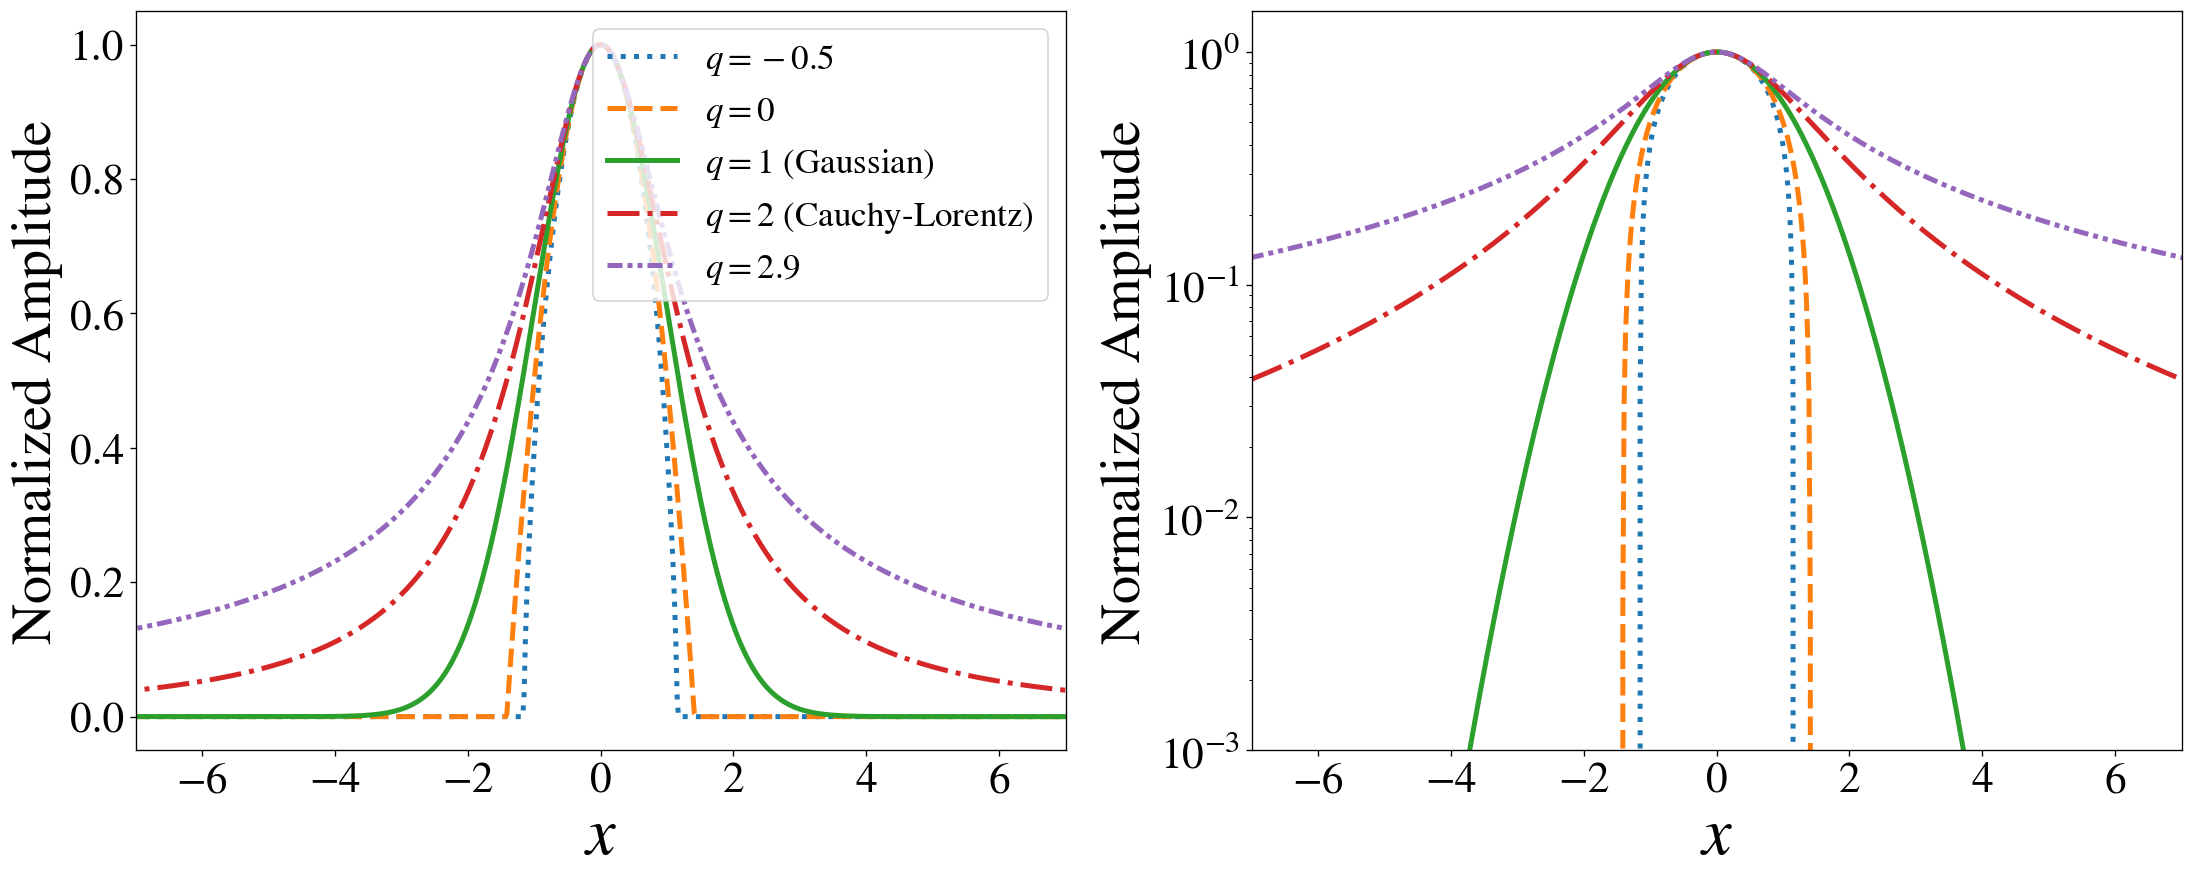
\includegraphics[width=\textwidth,keepaspectratio]{chapter6/qgaussians.png}
    \caption{Several q-Gaussian distributions for different q parameters normalized to unit amplitude and with a scale parameter of $\sigma=1$. The left plot uses linear scaling and the right one uses logarithmic scaling for the y-axis.}
    \label{fig:qgaussians}
\end{figure}


\section{\label{sec:static_high}Static Tune Scans at Different Intensities}

Section \ref{sec:static_low} showed how static tune scans are a useful tool to verify if the resonance compensation scheme is beneficial to the Recycler Ring. Nevertheless, these studies in Ch. \ref{sec:ch4} were done at low intensities. It is of interest to go to higher intensities and perform these static tune scans with a larger tune spread. Figure \ref{fig:static14_bare} shows a static tune scan crossing the $3Q_x$ line with no compensation at an intensity of approximately 4.5e10 ppb (14 BTs) and a set vertical tune of $Q_y=24.44$. The beam survival ratio drops dramatically after the 25.37 tune as the beam starts hitting the resonance line. At the same time, the beam size grows exponentially. If this plot is compared to the low-intensity case from Fig. \ref{fig:static2_ipm}, one can see that the losses start earlier at high intensities due to the fact that the space charge tune spread is larger for this case. The beam size growth is also enhanced at high intensities. With large tune spreads, the beam survival ratio plots get more messy given that beam can be operating on top of multiple resonance lines at once, and basically there is no stable beam. This can be seen for tunes lower than 25.35 in Fig. \ref{fig:static14_bare}. This fact is aggravated by the fact that the transverse dampers are on for this particular experiment, but they have been fine-tuned to operate in another tune region. 

\begin{figure}[H]
    \centering
    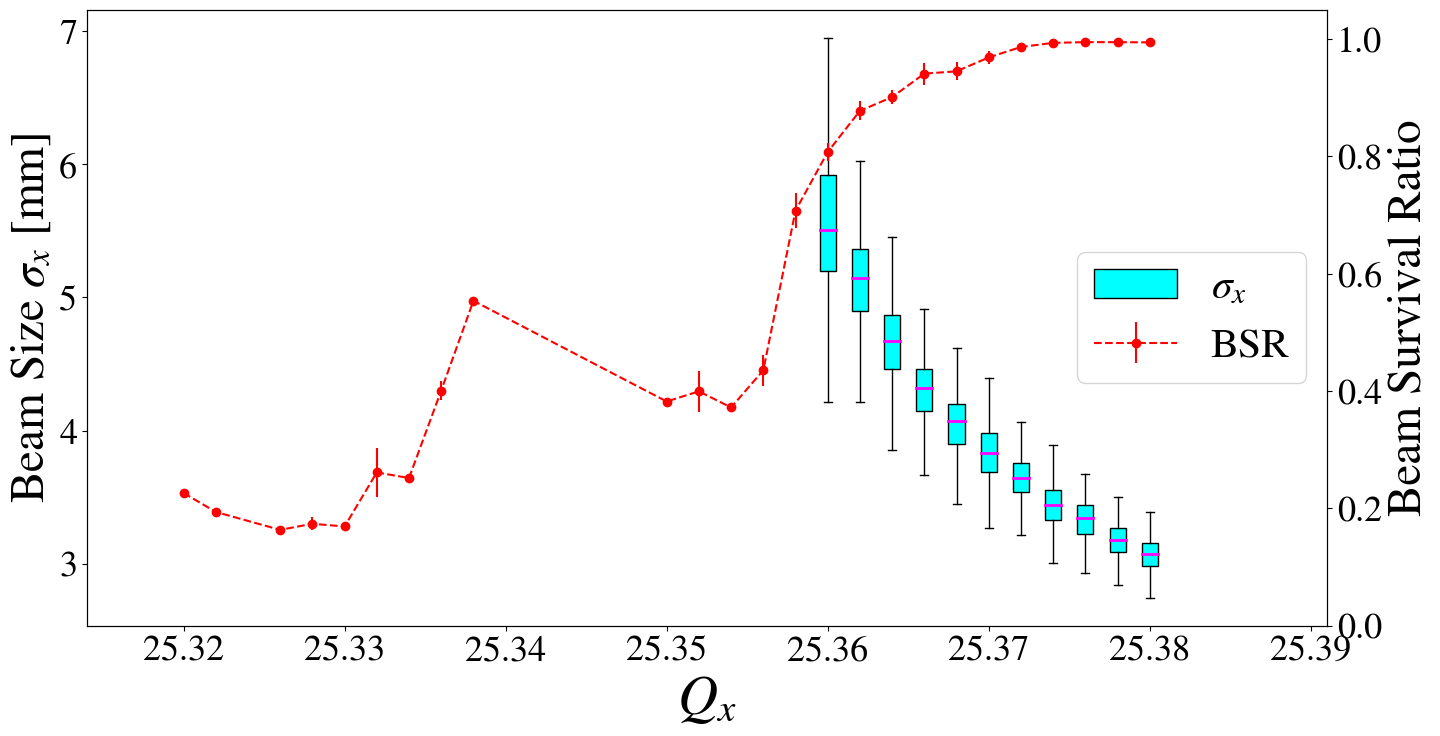
\includegraphics[width=\columnwidth]{chapter6/static14turns_BARE_dampersON.png}
    \caption{Static tune scan at an equivalent intensity of 14 Booster turns or approximately 4.5e10 ppb with no $3Q_x$ compensation and transverse dampers on.}
    \label{fig:static14_bare}
\end{figure}

In Ch. \ref{sec:ch4} it was shown that when the $3Q_x$ compensation was introduced, this helped improve the beam survival ratio close to and on top of the resonance line. Figures \ref{fig:static2_scatter}, \ref{fig:static8_scatter} and \ref{fig:static14_scatter} show what happens to the beam survival ratio and the beam size at different intensities during these static tune scans. It is worth pointing out that for these particular measurements the transverse dampers were turned off. A deeper discussion into the effect of transverse dampers is done in Sec. \ref{sec:ch6dampers}. Additionally, the color map of the scatter plot utilized for these figures represents the decimated turn number of the data point. Blue means that the data point happened earlier in the cycle---closer to injection---and yellow means it happened later in the cycle. A decimated number of turns of 1024 corresponds to 65000 real turns in the machine.

\begin{figure}[H]
    \centering
    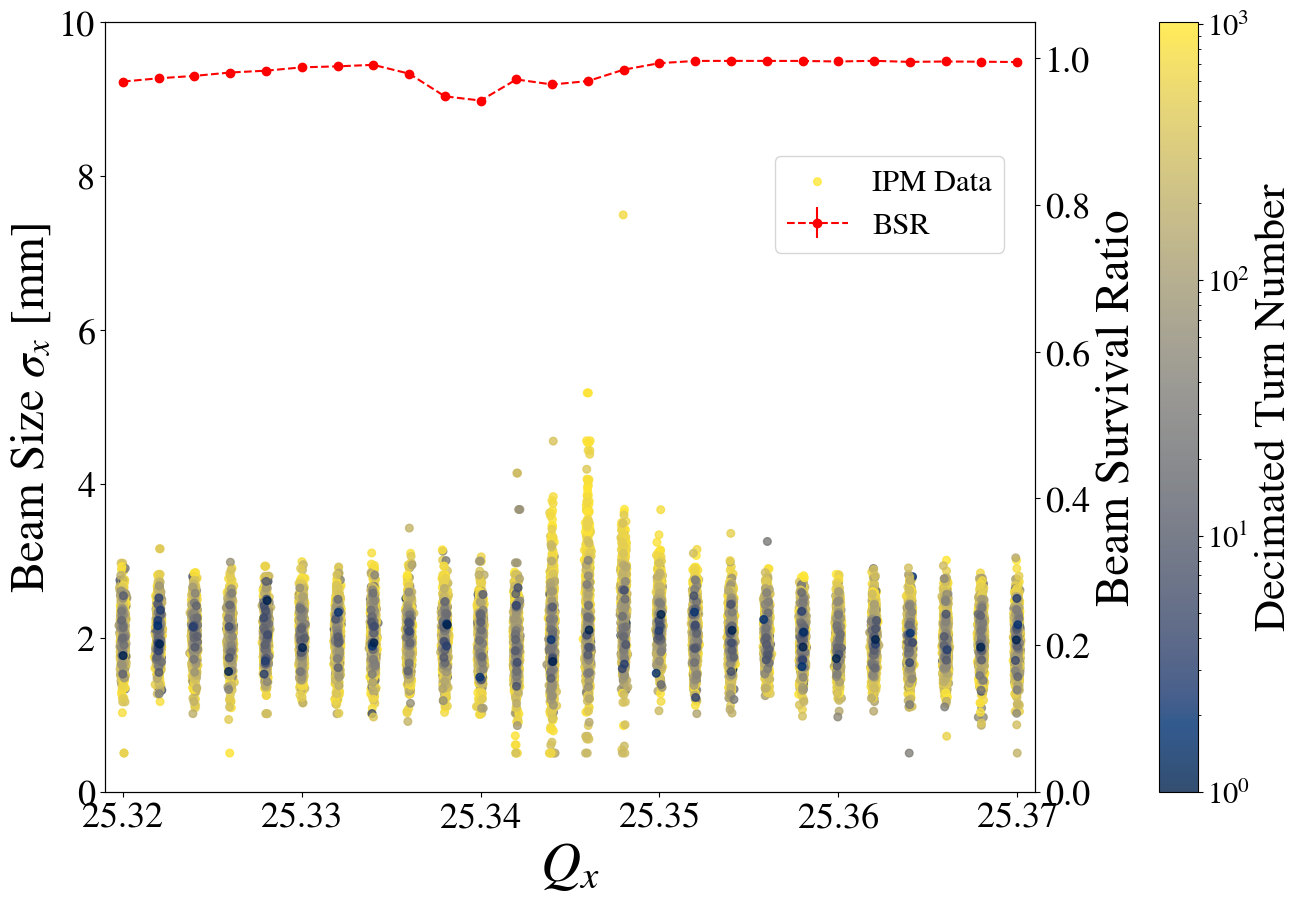
\includegraphics[width=\columnwidth]{chapter6/static2turns_dampersOFF.png}
    \caption{Static tune scan at an equivalent intensity of 2 Booster turns or approximately 0.5e10 ppb.}
    \label{fig:static2_scatter}
\end{figure}

The data for Fig. \ref{fig:static2_scatter} has already been shown in Figs. \ref{fig:static2_ipm_comp} and \ref{fig:static2_emit_comp}. Nevertheless, it is of interest to reference it again as the base case to compare against for the high intensity cases. In particular, Fig. \ref{fig:static2_scatter} shows the beam size and beam survival ratio as a function of horizontal tune and decimated turn number. When compensated for, more than 95\% of the beam survives on top of the $3Q_x$ resonance for 0.8 seconds. Nevertheless, there is some beam size growth when operating close to a set tune of $Q_x=25.345$, which is where the $3Q_x=76$ resonance lies. This beam size growth does not happen immediately but after many turns, as seen by the yellow color on large beam sizes. Nevertheless, out of this particular region there is no noticeable beam size growth for other tune values.

\begin{figure}[H]
    \centering
    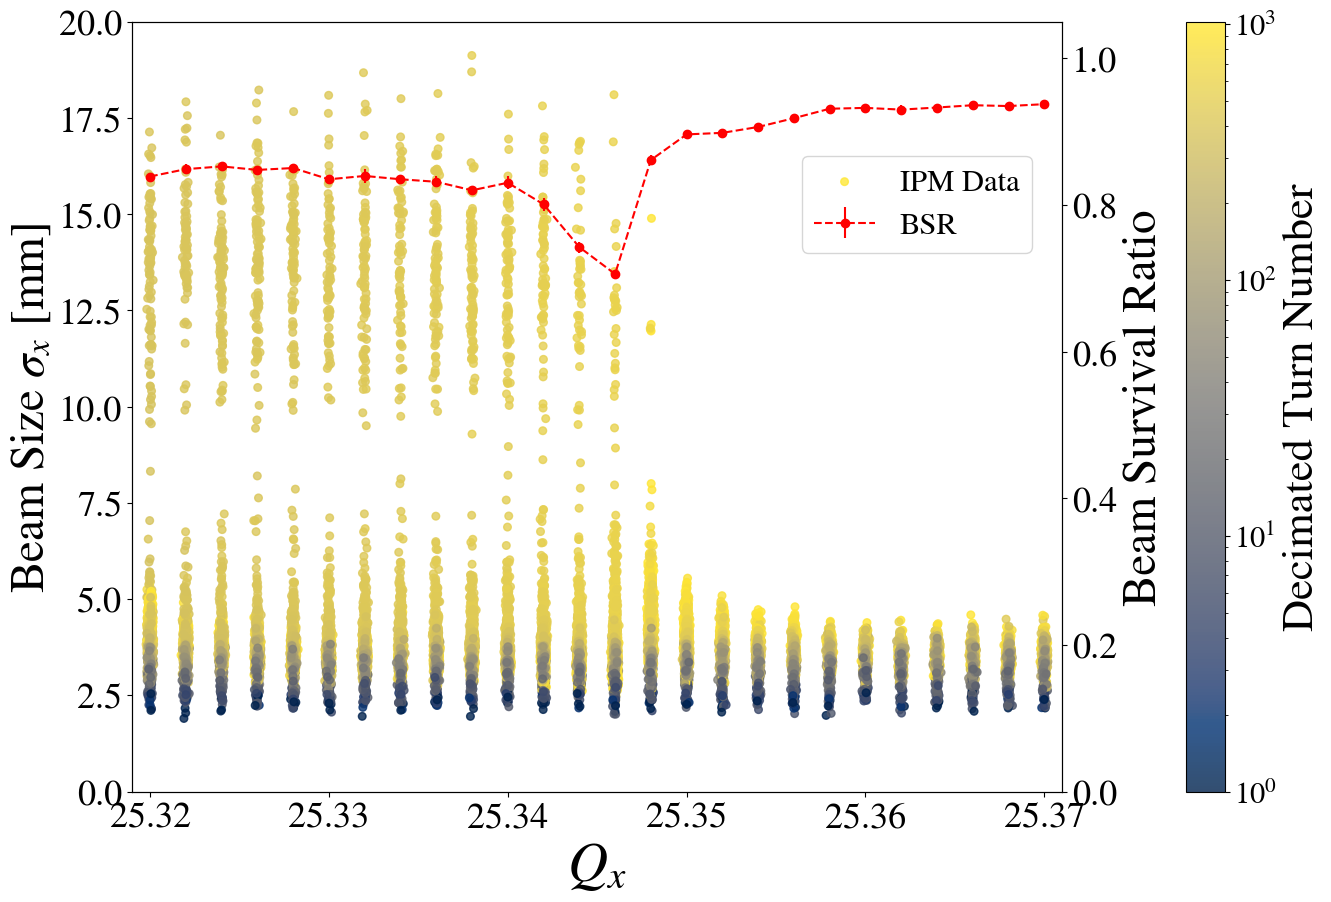
\includegraphics[width=\columnwidth]{chapter6/static8turns_dampersOFF.png}
    \caption{Static tune scan at an equivalent intensity of 8 Booster turns or approximately 3e10 ppb.}
    \label{fig:static8_scatter}
\end{figure}

Figure \ref{fig:static8_scatter} shows a static tune scan done at a higher intensity than the one in Fig. \ref{fig:static2_scatter}, i.e., 3e10 ppb which is approximately 6 times larger. From Fig. \ref{fig:tunespread}, the corresponding space charge tune spread corresponds to approximately 0.015. Therefore, the beam size growth and losses should start earlier in the scan. This can be seen on Fig. \ref{fig:static8_scatter} as compared to the low intensity case. The other feature to note is the beam size growth at every tune value for the scan. The beam is injected and undergoes some mechanism that leads to beam size growth. This mechanism is related to space charge given that it is not present at low intensities. Furthermore, it can be seen that the beam size grows as a function of tune before leading to a big dip in the beam survival ratio. At this point the beam size is large enough to be hitting the aperture of the Recycler. Ultimately, it is interesting to see the interplay between space charge, beam size growth and physical aperture of the machine.      

\begin{figure}[H]
    \centering
    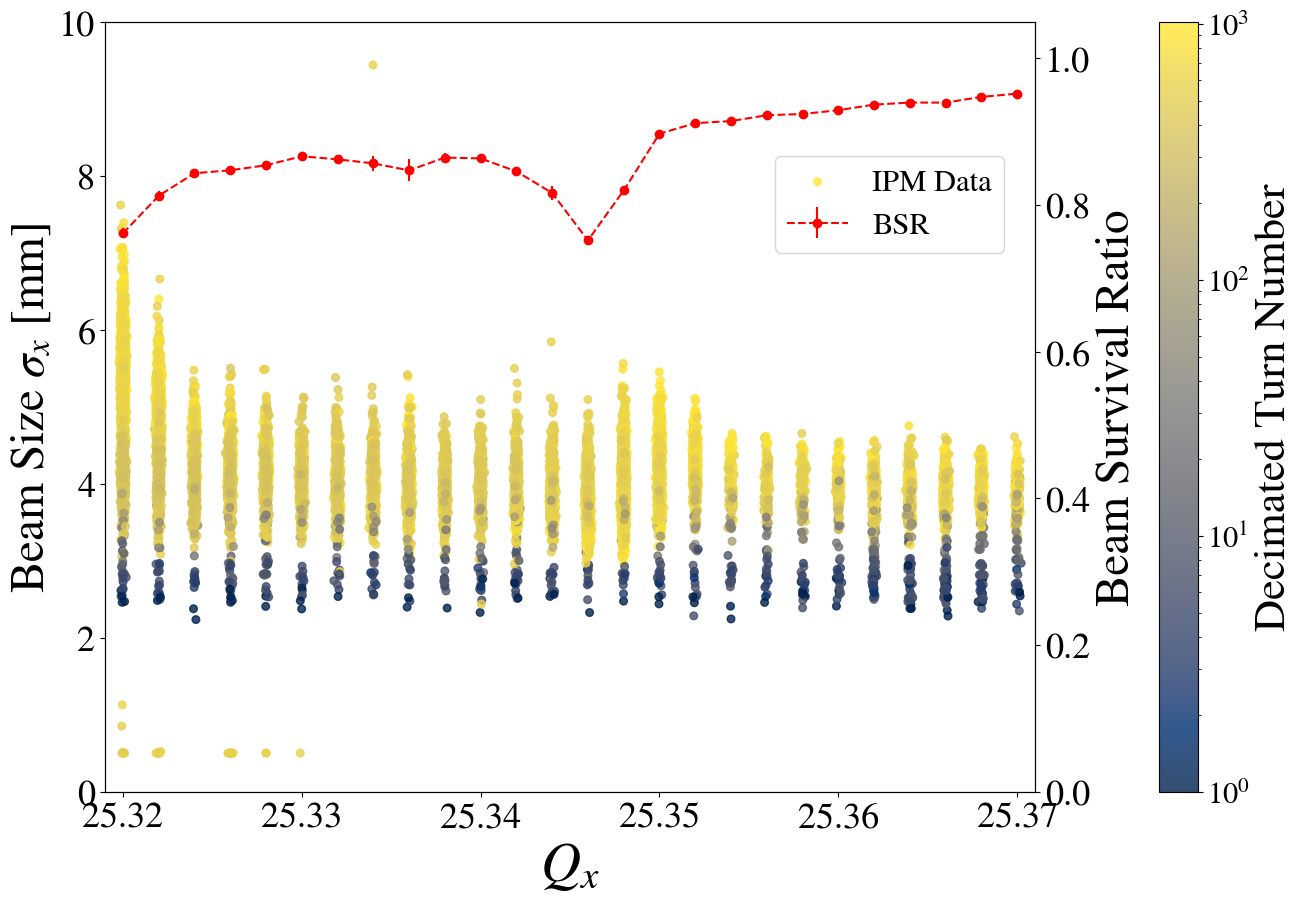
\includegraphics[width=\columnwidth]{chapter6/static14turns_dampersOFF.png}
    \caption{Static tune scan at an equivalent intensity of 14 Booster turns or approximately 4.5e10 ppb.}
    \label{fig:static14_scatter}
\end{figure}

Going to almost double of the previous intensity, Fig. \ref{fig:static14_scatter} shows a static tune scan done for an intensity of 5e10 ppb (particles per bunch). While the intensity is almost doubled, the tune spread only jumps to 0.02. This is due to the fact that the emittance grows exponentially, and the tune spread saturates as shown in Fig. \ref{fig:tunespread}. This small change in tune shift explains why Figs. \ref{fig:static8_scatter} and \ref{fig:static14_scatter} exhibit very similar behaviors. Nevertheless, a closer look shows that the injection beam size is slightly higher for this higher intensity, as expected from the emittance data shown in Fig. \ref{fig:tunespread}. Furthermore, the beam survival ratio also decreases slightly due to this. 

\begin{figure}[H]
    \centering
    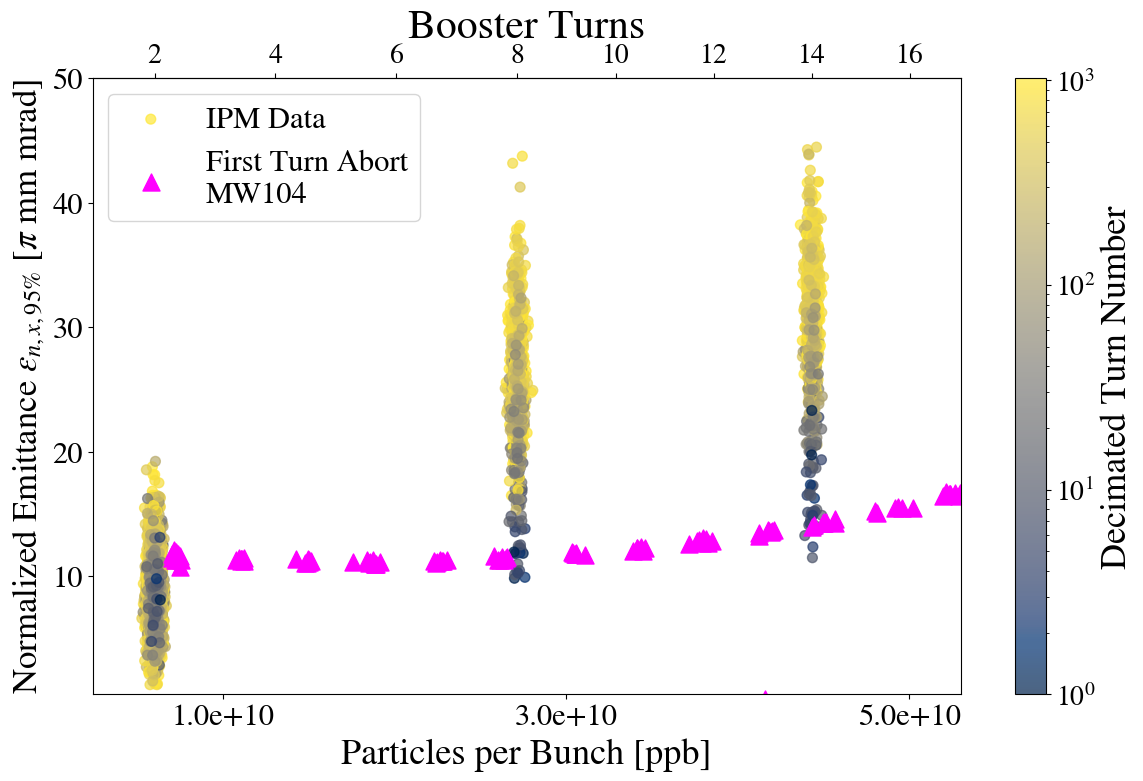
\includegraphics[width=\columnwidth]{chapter6/25370_scatter.png}
    \caption{IPM data and multi-wire first turn abort data for $Q_x=25.370$ at different intensities.}
    \label{fig:25370_scatter}
\end{figure}

Figure \ref{fig:25370_scatter} shows the comparison between emittance evolution data at these different intensities, as calculated from Eq. \ref{eq:emittance}. A set tune of $Q_x=25.37$ was used for comparison. On this plot, first-turn-abort emittances are also plotted as fuchsia triangles. Ideally, these emittances calculated from multiwire data should correspond to the emittances calculated from the IPM data. At low intensities, the emittances from the IPM data are centered around the multiwire value. At higher intensities, the IPM data for the initial number of turns coincides with the first-turn-abort data. Nevertheless, once injected the beam emittance grows as it circulates many turns around the ring. This growth can ultimately lead to beam loss. Ultimately, The IPM is a very useful tool in order to characterize these effects stemming from space charge. The multi-wires could not survive such high intensities for many turns. 

\begin{figure}[H]
    \centering
    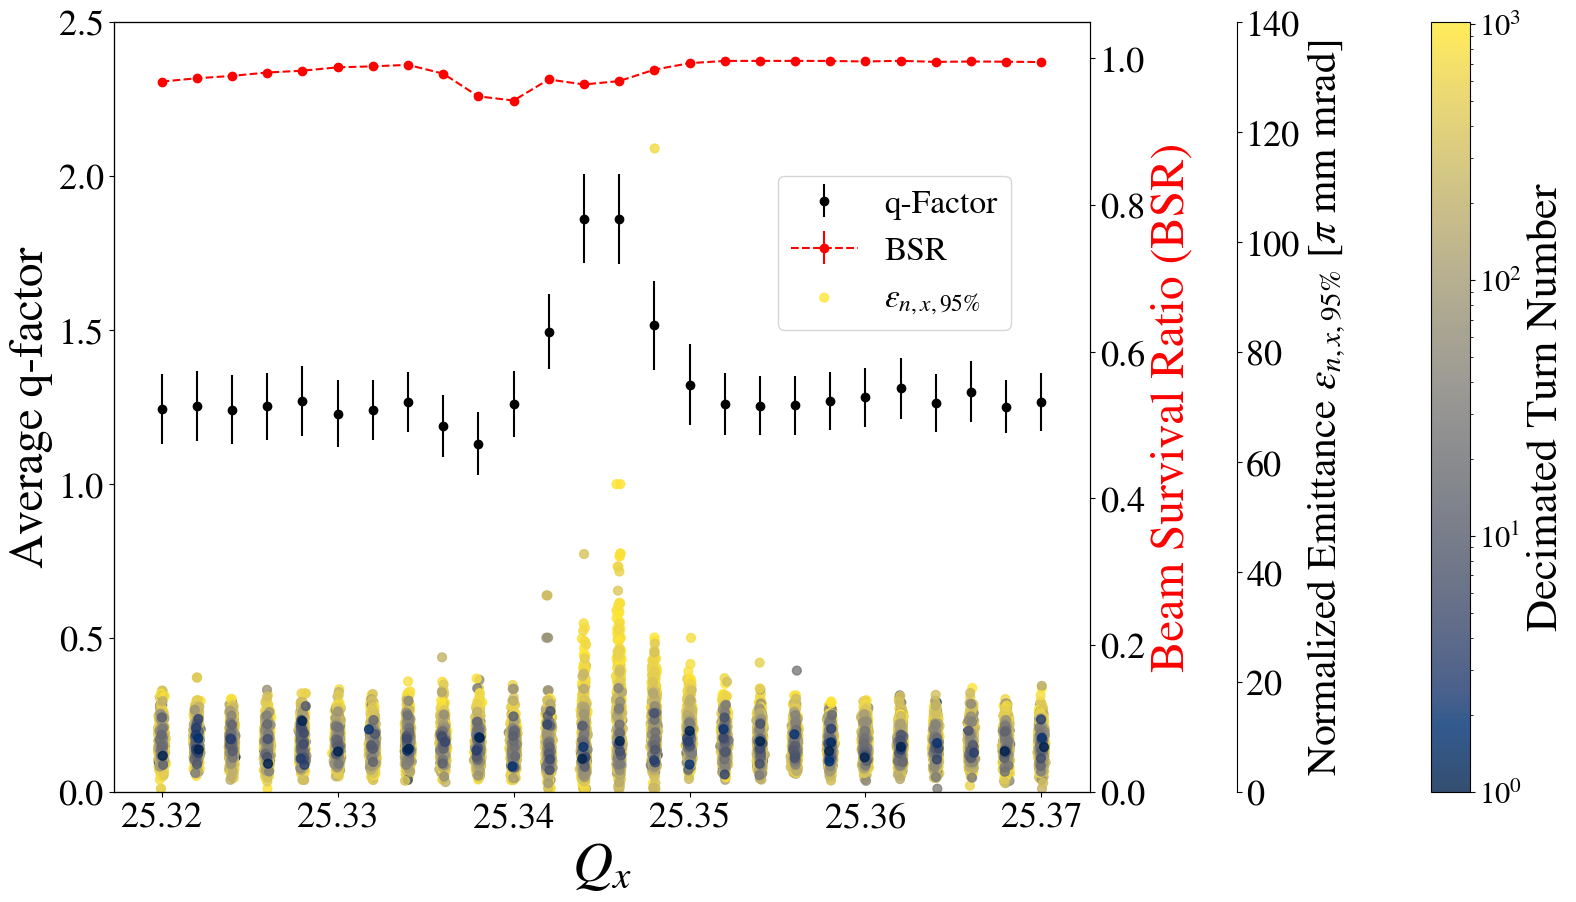
\includegraphics[width=\columnwidth]{chapter6/static2turns_emittance_dampersOFF.png}
    \caption{Static tune scan with beam survival ratio (BSR), average q-factor for the q-Gaussian fits, and beam size $\sigma_x$ at an equivalent intensity of 2 Booster turns or approximately 0.5e10 ppb.}
    \label{fig:static2_q}
\end{figure}

Going a step further with IPM data, one can use q-Gaussian distributions in order to fit raw data from the beam profile. Using Eq. \ref{eq:qgaussian} to fit IPM data, the $q$ parameter can be extracted in order to characterize the beam tails. Figures \ref{fig:static2_q}, \ref{fig:static8_q} and \ref{fig:static14_q} show a plot of the average $q$ values at each tune for the different intensities. This $q$ values should quantify how populated the tails are. A priori, one would not expect the tails to be under populated---all $q$ values should be above 1, $q>1$. Figures \ref{fig:static2_q}, \ref{fig:static8_q} and \ref{fig:static14_q} also plot the beam survival ratio and horizontal normalized emittance calculated from IPM data. Analyzing all of these quantities together helps understand the loss mechanism that brings down the beam survival ratio. 

For low intensities, it has been shown that the beam survival ratio improves when the $3Q_x$ compensation is introduced. Figure \ref{fig:static2_q} takes a closer look at how the small losses develop through the $q$ factor. Close to $Q_x=25.345$ the beam survival ratio drops slightly, at the same time the normalized emittance and the average $q$-factor increase. In particular, the emittance increases after tens of thousands of turns in the Recycler. While the sextupole term that feeds the $3Q_x$ line has been cancelled out, there are still higher order terms that feed the resonance line causing emittance growth and beam loss in this region. Furthermore, the beam tails are populated in this region---the average $q$ factor increases. Therefore, a combination of emittance growth and tail population from the resonance line explain the beam losses in this region. It is also worth pointing out that average $q$-factor for these fits is slightly above 1.0, around 1.2, meaning that the raw data from the IPM system is not necessarily Gaussian. This does not happen in Figs. \ref{fig:static8_q} and \ref{fig:static14_q}, where $q$ values before the resonance are centered around 1.0. It is worth reminding the reader that the IPM system is designed to operate at higher intensities. 

\begin{figure}[H]
    \centering
    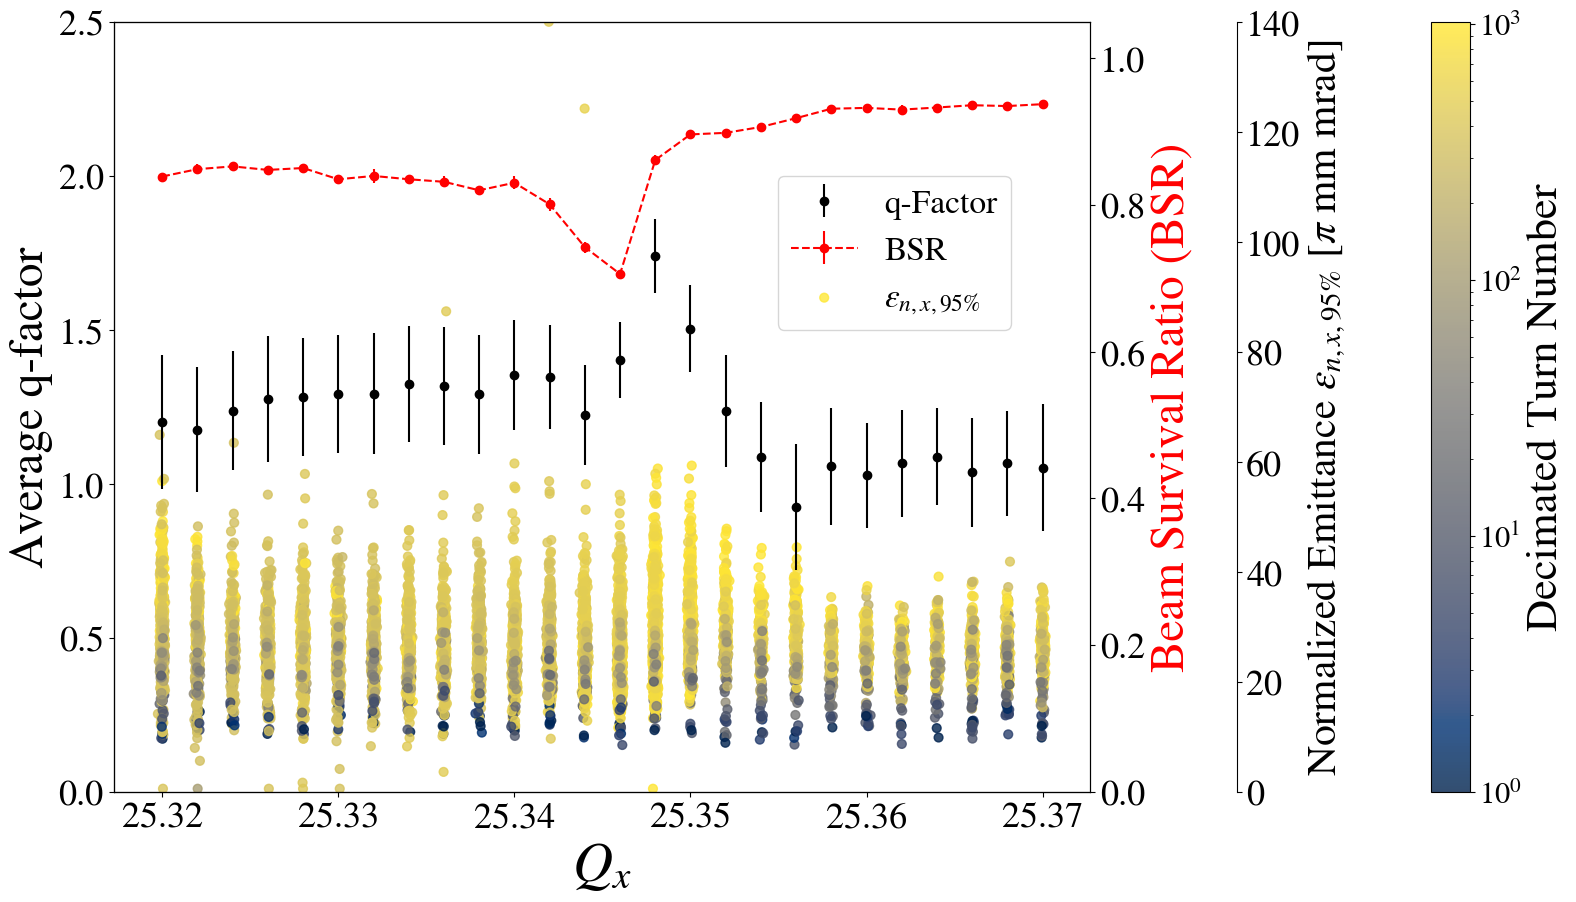
\includegraphics[width=\columnwidth]{chapter6/static8turns_emittance_dampersOFF.png}
    \caption{Static tune scan with beam survival ratio (BSR), average q-factor for the q-Gaussian fits, and beam size $\sigma_x$ at an equivalent intensity of 8 Booster turns or approximately 3e10 ppb.}
    \label{fig:static8_q}
\end{figure}

According to Ref. \cite{rr0} the transverse acceptance of the Recycler Ring is 40 $\pi$ mm mrad. Taking a closer look into the emittance plot of Fig. \ref{fig:static2_q}, it can be seen that when the normalized emittance starts hitting this value, that is where losses start to appear. Figure \ref{fig:static8_q} shows how at injection---for the first couple of initial turns of 3e10 ppb beam---the emittance is well below 40 $\pi$ mm mrad. Nevertheless, as the beam circulates around the Recycler Ring, the emittance grows close to the acceptance of the machine. Given that this is the 95\% emittance there is still beam outside this phase space region, particularly in the tails of the beam. This is why the beam survival ratio is not necessarily close to 1.0, even far from the resonance. This can also be seen at a higher intensity of 4.5e10 ppb beam through Fig. \ref{fig:static14_q}. While the injection emittance is slightly higher, the beam still grows all the way to the limit of acceptance of the machine. While the beam emittance grows, the space charge tune spread in the Recycler is decreasing from its original value. Close to the remnants of the resonance, there is a small dip in the beam survival ratio caused by the beam emittance increasing. As long as the emittance comes close to the acceptance of the machine, there will be losses from beam tail particles hitting the aperture of the machine. 

\begin{figure}[H]
    \centering
    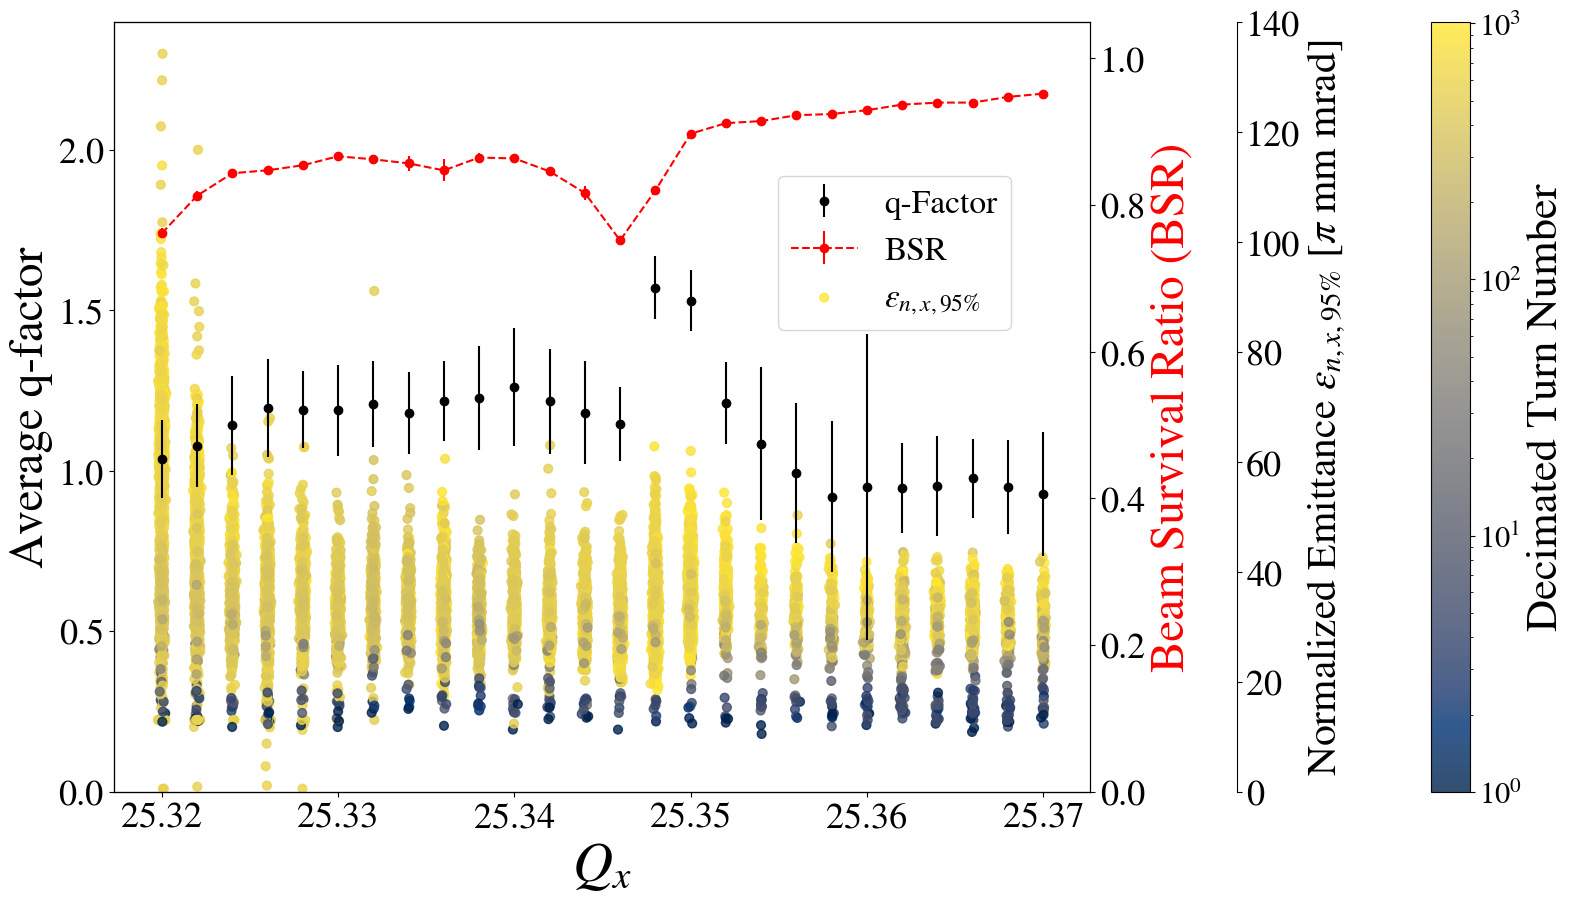
\includegraphics[width=\columnwidth]{chapter6/static14turns_emittance_dampersOFF.png}
    \caption{Static tune scan with beam survival ratio (BSR), average q-factor for the q-Gaussian fits, and beam size $\sigma_x$ at an equivalent intensity of 14 Booster turns or approximately 4.5e10 ppb.}
    \label{fig:static14_q}
\end{figure}

The other important feature from the plots shown in Figs. \ref{fig:static8_q} and \ref{fig:static14_q} is the average $q$-factor behavior. Close to $Q_x=25.35$, the average $q$-factor increases. This coincides with a dip in the beam survival ratio. Given that the beam is already on the limit of the acceptance, any increase in the beam tail population will inevitably lead to beam loss. This is what Figs. \ref{fig:static8_q} and \ref{fig:static14_q} are essentially showing. A point is reached where there is no more space in the beam pipe to accommodate more beam tails, therefore, any tail population mechanism will just lead to beam loss. After this point, if the beam is wide enough there are no beam tails given that they are being collimated by the beam pipe itself, and everything is just the beam core. This is what happens for tunes left of the resonance line. Essentially, while there exists emittance growth all the way to the limits of the machine, any beam tail population mechanism will just lead to beam loss. 

\section{\label{sec:ch6dampers}Effect of Transverse Dampers}

As hinted at previously, the transverse dampers play a role in the quality of resonance compensation. The transverse dampers at the Recycler Ring are used to suppress the coupled bunch beam instability from the slip-stacked beam \cite{dampers1,dampers2}. This system consists of a BPM pickup, input filters, digital signal processing, output amplifiers and stripline kickers. One set for the horizontal direction, and another one for the vertical. The general knobs to tune the damper system include timing delays and gain settings. For the experiments shown previously, the dampers were completely turned off. Nevertheless, some experiments were done with the damper system turned on, in order to observe its effect. Figures \ref{fig:static2_dampersON} and \ref{fig:static2_dampersOFF} show a comparison between static tune scans done at low intensity (0.5e10 ppb) with dampers on and off.

From just looking at Fig. \ref{fig:static2_dampersON} one could conclude that the resonance compensation does not fully work because only 60\% of beam survives close to the resonance. Nevertheless, these losses go away when the dampers are turned off for Fig. \ref{fig:static2_dampersOFF}.  

\begin{figure}[H]
    \centering
    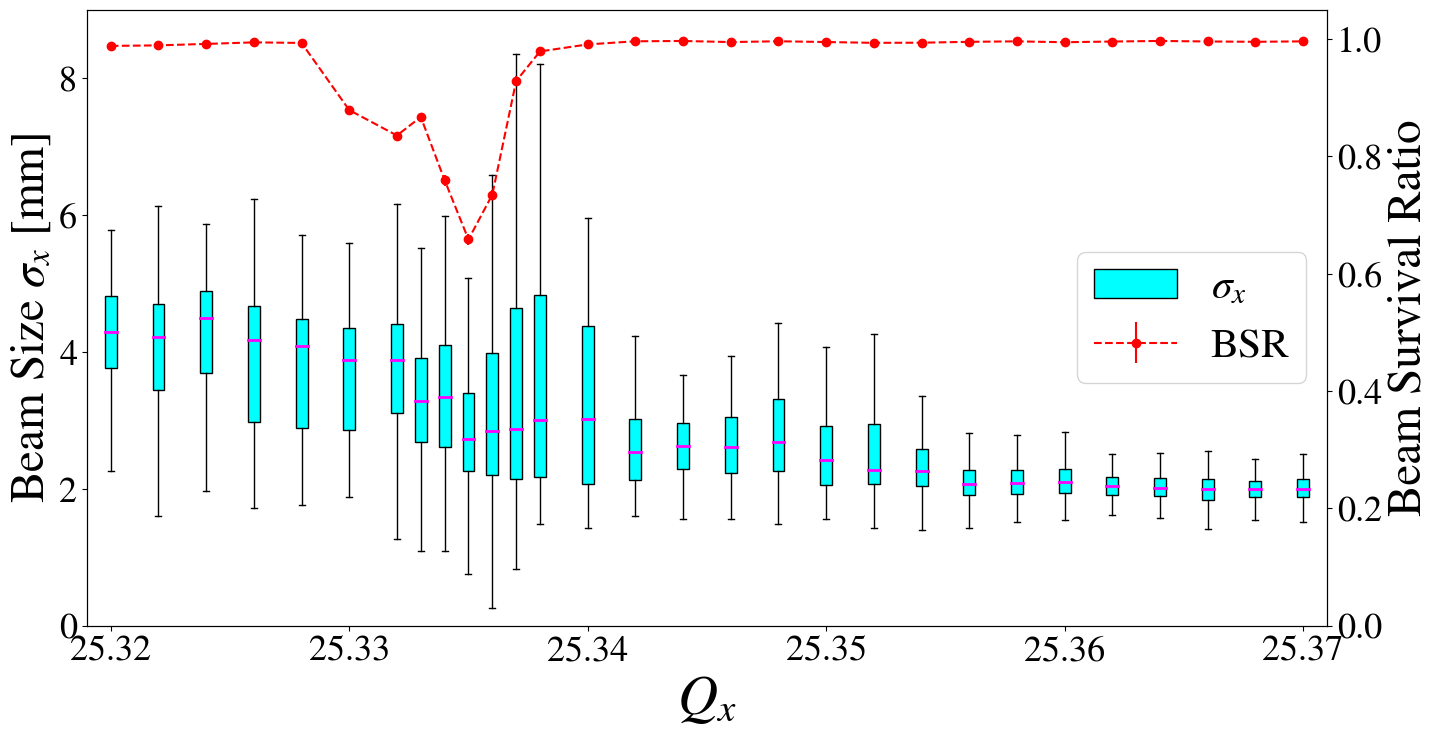
\includegraphics[width=\columnwidth]{chapter6/static2turns_ipm_dampersON.png}
    \caption{Static tune scan with beam survival ratio and IPM data box plots with $3Q_x$ compensation, transverse dampers ON and 2 Booster Turns of equivalent intensity or approximately 0.5e10 ppb.}
    \label{fig:static2_dampersON}
\end{figure}

\begin{figure}[H]
    \centering
    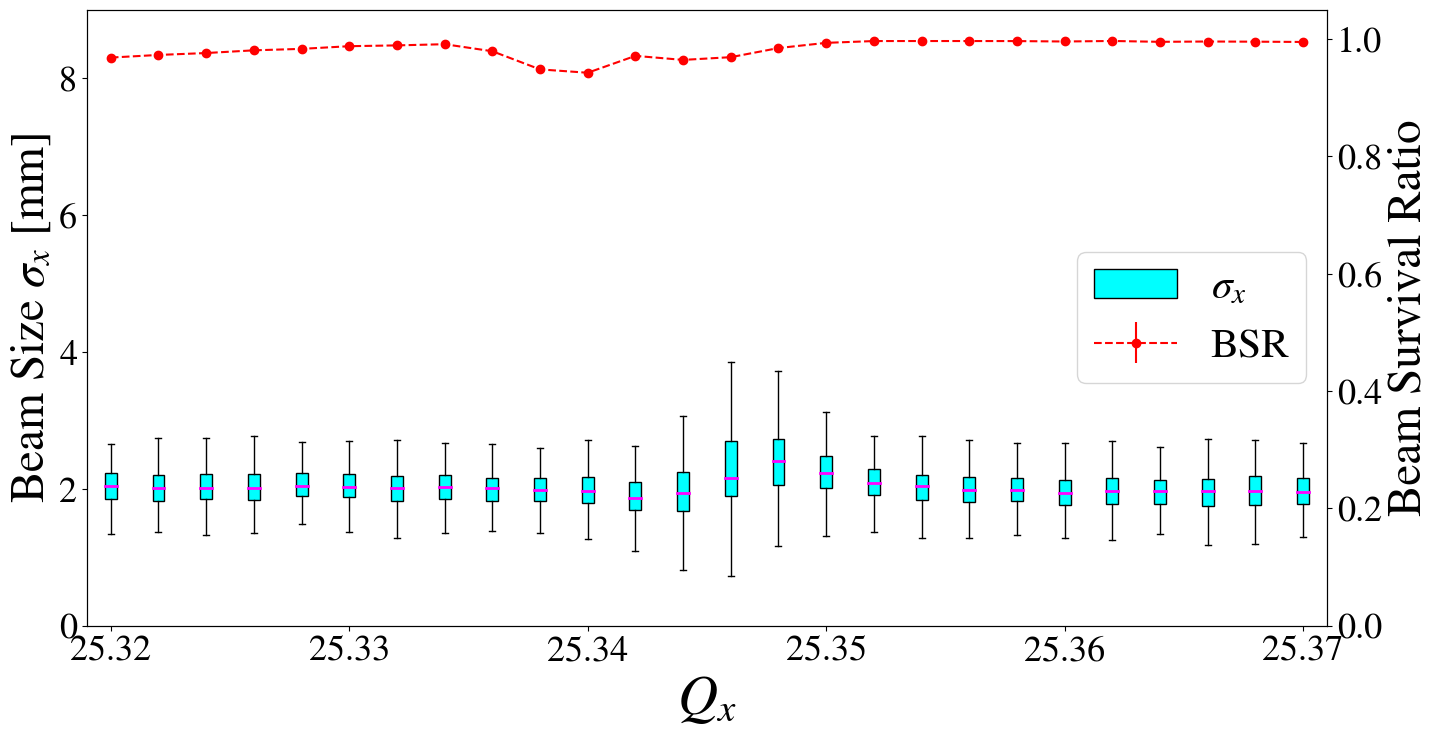
\includegraphics[width=\columnwidth]{chapter6/static2turns_ipm_dampersOFF.png}
    \caption{Static tune scan with beam survival ratio and IPM data box plots with $3Q_x$ compensation, transverse dampers OFF and 2 Booster Turns of equivalent intensity or approximately 0.5e10 ppb.}
    \label{fig:static2_dampersOFF}
\end{figure}

\begin{figure}[H]
    \centering
    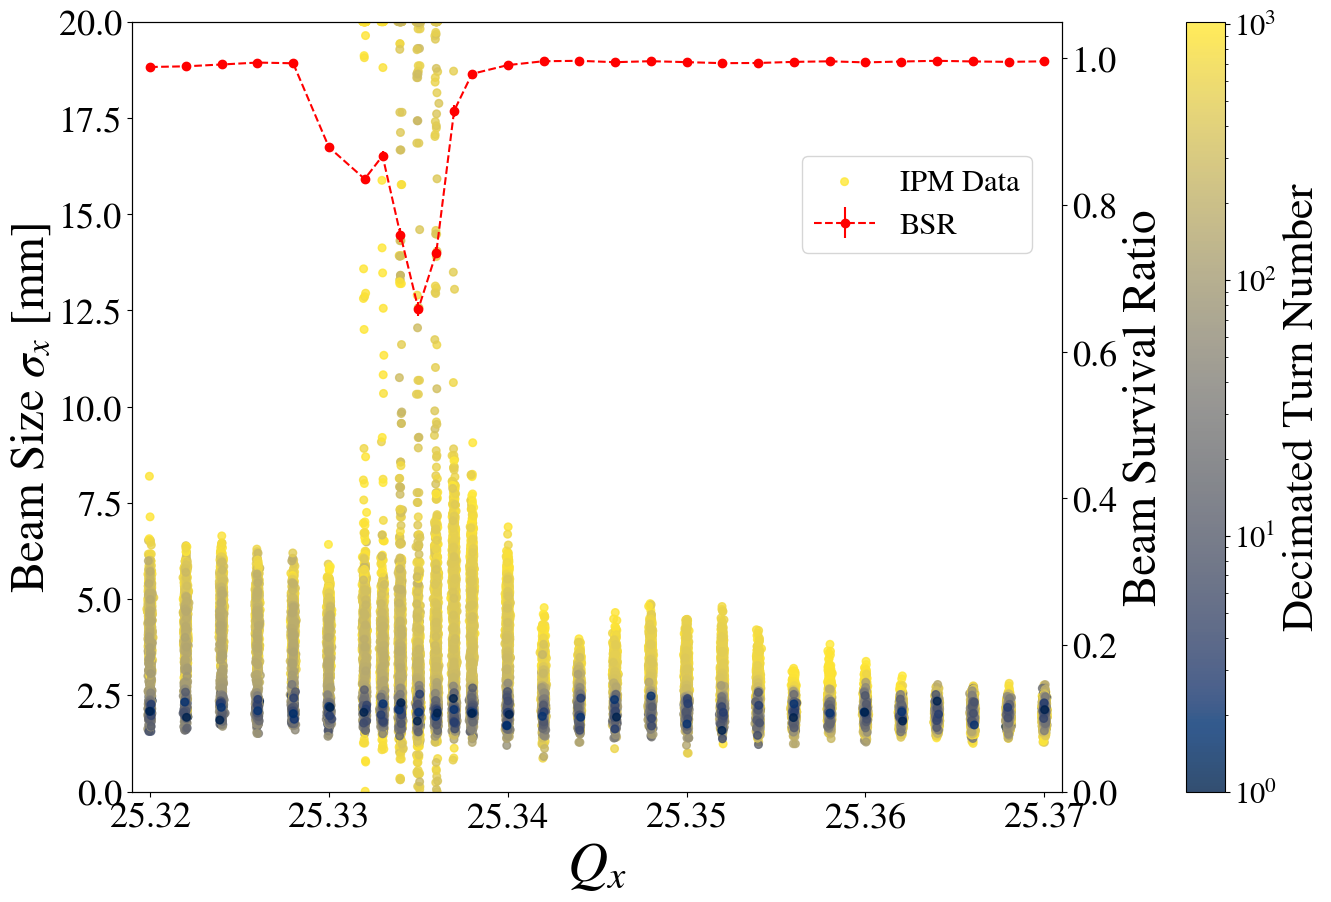
\includegraphics[width=\columnwidth]{chapter6/static2turns_dampersON.png}
    \caption{Static tune scan with beam survival ratio and IPM data scatter plots with $3Q_x$ compensation, transverse dampers ON and 2 Booster Turns of equivalent intensity or approximately 0.5e10 ppb.}
    \label{fig:static2_scatter_dampersON}
\end{figure}